\label{sec:peak_detection}
In this section a simplified tone-locating algorithm will be implemented by peak amplitude detection.
The algorithm is tested with the specifications given in section \ref{sec:testspec}.
%The integration is validated according to the test specifications in \ref{ch3}
\subsection{Implementation of peak detection}
To figure out which single tone is being played in a given audio file at a given time, the STFT is analysed, and the peak amplitude of a given time is detected.
The visualization of this is a plot of the peaks in the output spectrogram over time.
\\ \\
The frequency with the highest amplitude, and henceforth the largest amount of energy, is the most represented frequency. 
In an audio file this will be the frequency of the tone being played or one of the harmonics of this frequency, cf. chapter \ref{ch2}.
This assumption will hold as long as the signal-to-noise ratio, SNR, of the signal is not smaller than a given lower limit, which is further explored in chapter \ref{ch11}. \\
With the signal transformed by the STFT each segmented data set corresponds to a FFT of a given time, and hence finding the peak amplitude and the corresponding frequency makes it possible to determine the tone being played at a given time. Due to the trade-off between temporal and spectral resolutions stated in theorem \ref{theo:Heisenberg} the located frequency is an approximation, and hence the frequency needs to be compared with the frequencies that could be expected from the guitar.
The use of such ´´code book'' will make an approximation of the tone a possibility even though the spectral resolution is rather low.
\\ \\
To make sure that the amplitude actually is from a tone being played and not from noise in the signal, a check can be implemented in the algorithm such that the amplitude is set to $0$ if the amplitude is not larger than a given limit.\\
An algorithm for locating the frequency with the largest amplitude is described in algorithm \ref{alg:FIR}.
\begin{algorithm}[H]
\caption{Peak amplitude detection of the STFT}
\label{alg:FIR}
\begin{algorithmic}[1]
\Procedure{Compute peak amplitude}{$signal,f_s,FFTsize,X,limit$}
\State  $X$ = STFT($signal$) \Comment {STFT calculation in an array $X$}
\State $Y =$ linspace($0$, $f_s/2$, $FFTsize/2$) \Comment {Array of length $FFTsize/2$}
	\For {each $i$ in length of $X$}
		\State $A = \max(X[i])$ \Comment {Maximum amplitude for each FFT}
		\If {$A > limit$} \Comment {Checks if the amplitude is larger than a given limit}
			\State $freq\_pos[i] = $np.where$(X[i][:] == \max(X[i]))$ \Comment {Max amplitude}
		\Else
			\State $freq\_pos[i]$ = 0	
		\EndIf
		\If {$freq_pos[i]$ == 0}
			\State $max\_freq\_time = 0$
		\Else
			\State $max\_freq\_time = Y[freq\_pos]$
		\EndIf
	\EndFor
	\State Return $max\_freq\_time$
\EndProcedure
\end{algorithmic}
\end{algorithm}

%An argument coud be made for looking at the 3+ higest frequencies in the signal.
\subsection{Test of peak detection algorithm}
The algorithm is tested as stated by the specifications in section \ref{sec:testspec} by feeding an STFT of an audio file containing an $E_2$ tone being played on a guitar.
The expected result of this test is either the fundamental frequency of $82.41$ Hz or an harmonic of this as explained in chapter \ref{ch2}. The first two harmonics of $E_2$ are $82.41 \cdot 2 = 164.82$ Hz and $82.41 \cdot 3 = 247.23$ Hz.

\begin{figure}[H]
\centering
\begin{subfigure}{0.49\textwidth}
\centering
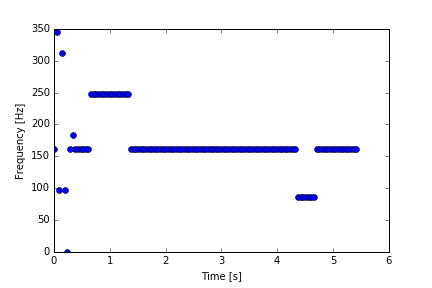
\includegraphics[width=\textwidth]{figures/peak_detection/peak_lim1.png}
\caption{}
\label{fig:freq_45dB_Amp_pass}

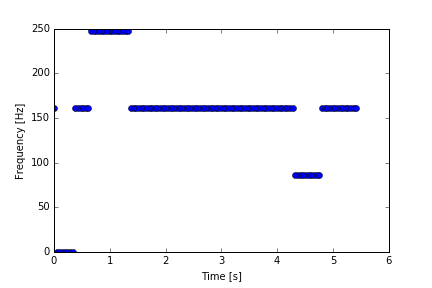
\includegraphics[width=\textwidth]{figures/peak_detection/peak_lim2.png}
\caption{}
\label{fig:freq_65dB_Amp_pass}

\end{subfigure}
\begin{subfigure}{0.49\textwidth}
\centering
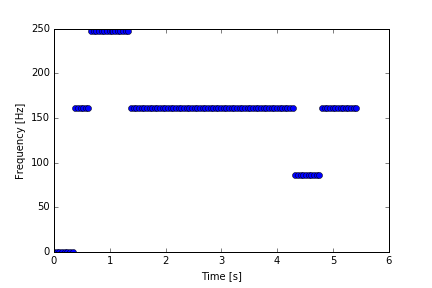
\includegraphics[width=\textwidth]{figures/peak_detection/peak_lim3.png}
\caption{}
\label{fig:freq_75dB_Amp_pass}

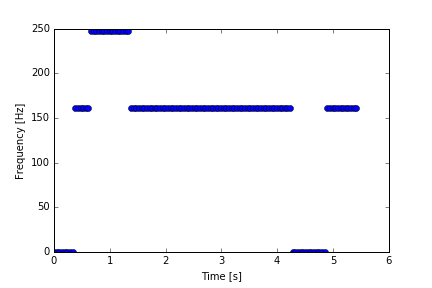
\includegraphics[width=\textwidth]{figures/peak_detection/peak_lim4.png}
\caption{}
\label{fig:freq_80dB_Amp_pass}

\end{subfigure}
\caption{Peak detection of spectrogram of $E_2$ with minimun amplitude representation of \textbf{(a)} 45 dB, \textbf{(b)} 65 dB, \textbf{(c)} 75 dB and \textbf{(d)} 80 dB.}
\label{fig:valdation_peak_detection}
\end{figure}
Figure \ref{fig:valdation_peak_detection} shows the effect of different cut-off limits. The most represented frequencies in figure \ref{fig:freq_45dB_Amp_pass} are $158.76$ Hz followed by $246.96$ Hz and $88.2$ Hz. 
Knowing that the tone being played is the $E_2$ with the previously mentioned fundamental frequency and harmonics, an error margin of around $6$ Hz between the expected output and the actual output can be seen. This can be due to either the guitar not playing a clean $E_2$ or the previously mentioned lack of resolution in frequency.
\\
With a low amplitude limit as shown in figure \ref{fig:freq_45dB_Amp_pass} none of the maximum amplitudes are removed. This in turn makes any noise in the system able to be represented as a peak even though nothing is being played by the guitar, seen by the first 0.5 seconds.
Figure \ref{fig:freq_80dB_Amp_pass} is more akin to an expected result as it does not show any spikes but the figure also only shows the harmonics of the $E_2$. Therefore, if the limit is too large, the tone being played is cut short when the amplitude of the tone gradually descends.
\\
To summarize, a compromise between letting noise pass the peak detection and cutting the tone short has to be made in order to make sure that the correct frequencies are located and the length of the tone is maintained. From this the implementation of the peak detection is found to work as intended.